\section{Basisløsninger}

%Jeg har endnu ikke fået gennemgået beviserne til de to sætninger ordentligt. de er bare stjålet fra jer andre.

Basisløsninger danner grundlaget for udregningen af den optimale løsning, hvilket beskrives og anvendes i Kapitel [indsæt ref til Kap simpLeX]. For at kunne beskrive netop basisløsninger er det nødvendigt først at introducere definitionen for \textbf{aktive betingelser}.%Ved ikke: Skal vi også bruge fed når ord introduceres i bindende tekst?

\begin{defn}[Aktive betingelser]
En betingelse siges at være \textbf{aktiv}, hvis det for en givet løsningsvektor $\vec{x}^*$ gælder, at $\vec{a}_i^T \vec{x}^* = b_i$.
\label{def:aktiv}
\end{defn}

Generelt bliver aktive betingelser brugt, da de for uligheder repræsenterer en grænse for de mulige løsninger i en given retning, mens de for ligheder blot beskriver, at betingelsen er opfyldt.
Yderligere anvendes skæringen mellem disse aktive betingelser, da den optimale løsning for lineære programmeringsproblemer findes i netop disse skæringer. Hvorfor dette netop er tilfældet bliver begrundet i Afsnit \ref{sec:ekstens}.

\begin{stn}[Lineært uafhængige rækker]
Lad $\vec{x}^* \in \mathds{R}^n$ og $I = \{i | \vec{a_i}^T \vec{x}^* = b_i\}$ være mængden af indekser for aktive betingelser. Da er følgende ækvivalent
\begin{enumerate}[label=(\alph*)]
\item Mængden $R_a =\{\vec{a_i}| i\in I\}$ består af $n$ elementer, som er lineært uafhængige.
\item Spannet $span(R_a) = \mathds{R}^n$.
\item Ligningssystemet $\vec{a_i}^T \vec{x}^* = b_i$, for $i \in I$ har en unik løsning.
\end{enumerate}
\label{stn:uniklosning}
\end{stn} %Ved ikke: Bør det siges at $\vec{a_i}$ repræcentere en række, eller er det underforstået i rapporten da den altid gør det?

\begin{proof}
(a) => (c): Lad $A$ være en $n \times n$ matrix bestående af rækkerne $\vec{a_i}^T \in R_a$, og antag at alle $\vec{a_i}$ er lineært uafhængige. 
Antag nu for modstrid at ligningssystemet $A\vec{x} = \vec{b}$, hvor $\vec{b}$ har indgangende $b_i$ for $i \in I$, har to løsninger. 
Da vil $A \vec{x} = \vec{b}$ og $A \vec{y} = \vec{b}$ hvorfor $A(\vec{x}-\vec{y}) = \vec{0}$.
Derfor må søjlerne enten være lineært afhængige, eller $(\vec{x}-\vec{y})= \vec{0}$.
Da der er $n$ lineært uafhængige rækker i $A$ må $rank(A) = n$, hvorfor alle søjler er lineært uafhængige, da $A$ er en $n \times n$ matrix.
Det medfører at $\vec{x}-\vec{y} = \vec{0}$, hvorfor det kan konkluderes at løsningen til ligningssystemet er unikt da $ \vec{x}=\vec{y}$, og der derved er bevist modstrid.
\\(c) => (a):Antag at der er en unik løsning til $A$ det medfører at $rank(A) = n$, hvorfor alle rækker må være lineært uafhængige, da $A$ er en $n \times n$ matrice. % s. 78-79 LinAlg
\\ (a) => (b): Da $R_a$ består af $n$ linært uafhængige $n$-dimentionelle vektorer, må $R_a$ udgøre en base for $\mathds{R}^n$, hvorfor $span(R_a) = \mathds{R}^n$.
\\ (b) => (a): Antag for modstrid, at vektorene i $R_a$ ikke er lineært uafhængige, da vil der eksistere en vektor $\vec{a_i'} \in R_a$ som er en linear kombination af de andre vektorer, der må derfor eksistere en vektor $A\vec{x} = \vec{0}$, hvor $\vec{x} \neq \vec{0}$, da det kun kan lade sig gøre hvis $\vec{x}$ er ortogonal med alle rækker i $A$, kan $\vec{x}$ ikke være en linear kombination af vektorene i $R_a$.
Hvorfor at $\vec{x} \notin span(R_a)$.
Derfor kan $span(R_a) \neq \mathds{R}^n$, hvorfor der er opstået modstrid.
\end{proof}

\begin{defn}[Basisløsning]
Lad $P$ være en polyide dannet af lineære bibetingelser, og lad $\vec{x}^*\in \mathds{R}^n$. Da er $\vec{x}^*$ en \textbf{basisløsning} hvis
\begin{enumerate}[label=(\alph*)]
\item Alle lighedskrav er aktive
\item Der er $n$ lineært uafhængige aktive krav
\end{enumerate}
og en \textbf{mulig basisløsning} hvis
\begin{enumerate}[label=(\alph*)]
\setcounter{enumi}{2}
\item $\vec{x}^*$ opfylder alle krav.
\end{enumerate}
\label{def:basislosning}
\end{defn}

Enhver bibetingelse udspænder et rum, for hvilket betingelsen er opfyldt. Skæringen, af de aktive betingelser, danner derved et rum, som er fællesmængden, af betingelsernes udspændte rum. Skæringen, af en mængde af aktive betingelser, svarer derved til den mulige mængde af disse betingelser. Dog gælder det for basisløsninger pr. Definition \ref{def:basislosning}, at der for en basisløsning $\vec{x}$ skal være $n$ lineært uafhængige aktive betingelser, hvorved en basisløsningen kun er et enkelt punkt, hvilket er bevist igennem Sætning \ref{stn:uniklosning}. %Ved ikke, er en vektor og et punkt det samme?

\begin{kor}[Endelig mængde af basisløsninger]
Givet en endelig mængde af bibetingelser, vil der kun eksistere en endelig mængde af basisløsninger og derved også kun en endelig mængde mulige basisløsninger.
\end{kor}

\begin{proof}
Betragt et lineært ligningssystem med $m$ uligheder og løsningsvektorer på formen $\vec{x} \in \mathds{R}^n$, hvor m er et endelige tal.
	Betragt da systemet af $n$ aktive uafhængige lineære uligheder udvalgt af de $m$ uligheder. Da vil dette system ifølge Sætning \ref{stn:uniklosning} kun have en løsning, og denne udvælgelse af uligheder giver derved kun en basisløsning. Da der kun er en endelig mængde af muligheder for at udtrække $n$ af $m$ uligheder på, vil der netop også kun være en endelig mængde af basisløsninger. Da mængden af mulige basisløsninger er en delmængde af mængden af basisløsninger, vil der også kun være en endelig mængde af mulige basisløsninger.
\end{proof}

\begin{stn}[Krav til basisløsninger]
Lad $A\vec{x}=b$, $\vec{x}\geq 0$, hvor $A$ er $m\times n$ matrix med lineært uafhængige rækker. Da er $\vec{x}^*\in \mathds{R}^n$ en basisløsning hvis og kun hvis $A\vec{x}^*=b, \vec{x}^* \geq 0$, og der eksisterer indekser $B(1), ..., B(m)$ således, at
\begin{enumerate}[label=(\alph*)]
\item kolonerne $A_{B(1)}, ..., A_{B(m)}$ er lineært uafhængige
\item $x_i = 0$ hvis $i \neq B(1),...,B(m)$
\end{enumerate}
\end{stn}

\begin{proof}
Lad $I$ være mængden af indeks for de lineære uafhængige løsninger$I={B(1),\dots,B(m)}$. per definition er $\vec{b}=\sum_{j=1}^{n}\vec{x_j}A_j$ som er summen af alle rækkerne gange en løsning som giver $\vec{b}$, det må være det samme som $b=\sum_{j\in I}^{n}\vec{x_j}A_j+\sum_{j\notin I}^{n}\vec{x_j}A_j$, som er summen af alle de lineære uafhængige rækker og deres løsninger lagt sammen med summen af de lineære afhængige rækker og deres løsninger, men $\vec{x_j}$ til de lineære uafhængige løsninger er er i følge sætningen $x_i = 0$ hvis $i \neq B(1),...,B(m)$ så derfor må ligningen blive $b=\sum_{j\in I}^{n}\vec{x_j}A_j+0$, så derfor må $\vec{x}$ være en basis løsning.
Modsat, hvis der antages at $\vec{x}$ er en basis løsning, så lad $x_{B(1)},\dots x_B(k)$ være alle ikke-nul komponenterne af $\vec{x}$. Eftersom $\vec{x}$ er en basis løsning, så må ligningssystemet af aktive bibetingelser $\sum_{i=1}^{n}A_ix_i=b$, hvor $x_i=0, i\neq B(1),\dots , B(k)$ have en unik løsning \textit{Pr. dif 2.2 i bert}, ligeledes må ligningen $\sum_{i=1}^{k}A_{B(i)}x_{B(i)}=b$ have en unik løsning og derfor må kolonerne $A_{B(1)}, ..., A_{B_(m)}$ være lineært uafhængige.\\
Eftersom kolonerne $A_{B(1)}, ..., A_{B_(m)}$ er lineært uafhængige, så må der $k\leq m$, \textit{herefter følger tingende af sætning 1.3(b) i bertsimas, som jeg ikke er helt sikker på endnu}
\end{proof}

\begin{alg}[Procedure for konstruktion af basisløsninger(bør ændres til procedure)]
\noindent 1. Vælg $m$ lineært uafhængige koloner $\vec{A}_{B(1)},\dots,\vec{A}_{B(m)}$\\
2. Lad $x_i=0 \,\forall i\neq\vec{A}_{B(1)},\dots,\vec{A}_{B(m)}$\\
3. Løs $A\vec{x}=\vec{b}$ for de ubekendte $x_{B(1)},\dots x_{B(m)}$
\end{alg}

\begin{comment}
Der mangler bare generelt bindetekst mellem sætninger, fra at korollar 6.12 skal introduceres til at kapitlet skal afsluttes og føres videre til naboløsninger
\end{comment}

\subsection{Naboløsninger}

Til den senere anvendelse af simpLeX metoden anvendes også \textbf{naboløsninger}, som er defineret i Definition \ref{def:nabo}. Undersøgelsen af naboløsninger i SimpLeX metoden som en metode til at reducere antallet af basisløsninger som skal undersøges når den optimale løsning findes. %Bør omformuleres, er kringlet. Ved ikke: Er det realt det der sker? Ved ikke: Skal SimpLeX staves med stort?

\begin{defn}[Naboløsninger]
	To basisløsninger i $\mathds{R}^n$ siges af være \textbf{naboløsninger}, hvis de deler præcis $n-1$ aktive lineært uafhængige bibetingelser.
	\label{def:nabo}
\end{defn}

Et eksempel på naboløsninger ses i Eksempel \ref{eks:nabo}.

\begin{eks}[Naboløsninger]
De to basisløsninger $\vec{p}=\rvect{4 & 4}^T$ og $\vec{q}=\rvect{10 & 2}^T$ set på Figur \ref{fig:nabo} er naboløsninger, da de har $n-1$ fælles aktive betingelser, hvilket for dette eksempel er 1 betingelse, nemlig betingelse (2). Basisløsningen $\vec{p}$ har (1) og (2) som aktive betingelser, mens $\vec{q}$ har (2) og (3) som aktive betingelser. %ved ikke, om nemlig bør slettes.
	
	\begin{center}
	\begin{tabular}{l	>{$}r<{$}	>{$}r<{$}	>{$}l<{$} r}
	Maksimer 		& 		4x_1	&	+3 x_2	& \\
	med hensyn til 	&  \ \ 	-2 x_1	& 	+4 x_2	& \leq 8 	& \quad (1)\\
					&  		x_1		& 	+3 x_2	& \leq 16	& \quad (2)\\
					&  \ \ 	x_1		& 			& \leq 10	& \quad (3)\\
	og $x_1 \geq 0$ (4), $x_2\geq 0$ (5).
	\end{tabular}
	\end{center}
	
	\begin{center}
	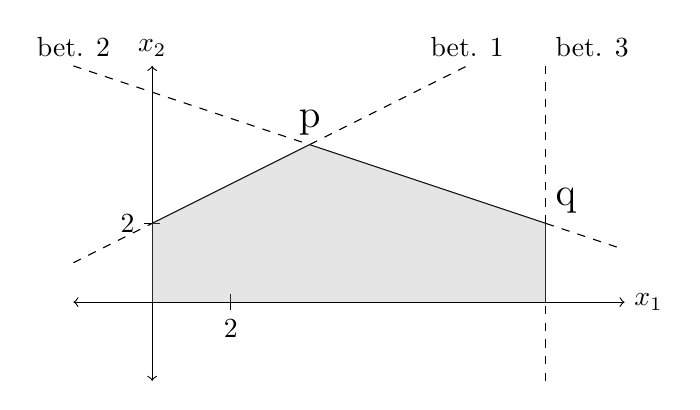
\begin{tikzpicture}
  %laver Grid. godt til når koordinater skal redigeres
  	%\draw[thin,gray!40] (-3,-1) grid (6,3); 
  %x-aksen
  	\draw[<->] (-1,0)--(6,0) node[right]{$x_1$};
  	%\draw[->,red] (2.5,0) -- (2.5,0.5);
  %y-aksen
  	\draw[<->] (0,-1)--(0,3) node[above]{$x_2$};
  	%\draw[->,red] (0,0.5) -- (0.5,0.5);
  	
  %akse-markeringer
  	%\node[left] (xakse) at (0,1) {2};
  	\draw[] (-0.1,1) -- (0.1,1) node[pos=0,left] {2};
  	\draw[] (1,-0.1) -- (1,0.1) node[pos=0,below] {2};
  	
  %ligning 1
	\draw[domain=-1:0,variable=\x,dashed] 	plot({\x},{0.5*\x+1});
	\draw[domain=0:2,variable=\x] 			plot({\x},{0.5*\x+1});
	\draw[domain=2:4,variable=\x,dashed] 	plot({\x},{0.5*\x+1}) node[above] {bet. 1};
  	%\draw[->,red] (1,1.5) -- (1.224,1.05);
	
  %ligning 2
  	\draw[domain=-1:2,variable=\x,dashed] 	plot({\x},{-(1/3)*\x+8/3}) node[above] at (-1,3) {bet. 2} ;
	\draw[domain=2:5,variable=\x] 			plot({\x},{-(1/3)*\x+8/3});
	\draw[domain=5:6,variable=\x,dashed] 	plot({\x},{-(1/3)*\x+8/3});
	%\draw[->,red] (3.5,1.5) -- (3.34,1.026);

  %ligning 3
  	\draw[domain=-1:0,variable=\y,dashed] 	plot({5},{\y});
	\draw[domain=0:1,variable=\y] 			plot({5},{\y});
	\draw[domain=1:3,variable=\y,dashed] 	plot({5},{\y}) node[above right] {bet. 3};
	%\draw[->,red] (5,0.5) -- (4.5,0.5);

  %nodes med navne på punkter
	\node[above] (p) at (2,2) {\Large p};
	\node[above right] (q) at (5,1) {\Large q};

  %løsningsmængden skraveret
	\fill[gray!80,nearly transparent] (0,0) -- (0,1) -- (2,2) -- (5,1) --(5,0) --  cycle;
\end{tikzpicture}
	\captionof{figure}{Løsningsmængde med naboløsninger $p$ og $q$.}
	\label{fig:nabo}
	\end{center}
\label{eks:nabo}
\end{eks}

%ved ikke: Må et afsnit slutte med et eksempel?




